\documentclass{nextgame2026} % Include author names
% \documentclass[anon]{nextgame2026} % Author names withheld
% \documentclass[final]{nextgame2026} % For Cam-ready

% The following packages are automatically loaded by jmlr.cls:
% amsmath, amssymb, natbib, graphicx, hyperref, algorithm2e

\usepackage{microtype}
\usepackage{booktabs}
\usepackage{mathtools}
\usepackage{enumitem}
\usepackage[capitalize,noabbrev]{cleveref}
\crefname{assumption}{Assumption}{Assumptions}
\Crefname{assumption}{Assumption}{Assumptions}

% jmlr already defines: theorem, lemma, proposition, corollary, definition, remark
% (all sharing one counter). Add assumption with its own counter.

\newtheorem{assumption}{Assumption}

\newcommand{\E}{\mathbb{E}}
\newcommand{\R}{\mathbb{R}}
\newcommand{\K}{\mathcal{K}}
\newcommand{\B}{\mathcal{B}}
\newcommand{\N}{\mathcal{N}}
\newcommand{\F}{\mathcal{F}}
\newcommand{\dist}{\operatorname{dist}}
\newcommand{\Proj}{\operatorname{Proj}}
\newcommand{\Var}{\operatorname{Var}}
\newcommand{\diag}{\operatorname{diag}}

\title[Basin Shaping for Opponent-Aware Learning]{Basin Shaping for Opponent-Aware Learning: Local Meta-MAPG Convergence with Restarts}

\optauthor{%
\Name{Yevhen Shcherbinin} \Email{eugene.shcherbinin@bloomsburytech.com}\\
\addr Bloomsbury Technology, London, UK \& London School of Economics, London, UK
\AND
\Name{Arina Redina} \Email{}\\
\addr University of Bristol, Bristol, UK \& Bloomsbury Technology, London, UK
\AND
\Name{Maxim Kalpin} \Email{}\\
\addr Bloomsbury Technology, London, UK \& Johannes Kepler University Linz, Austria
\AND
\Name{Vlad Kochetov} \Email{}\\
\addr Bloomsbury Technology, London, UK \& Odesa Polytechnic National University, Ukraine%
}

\begin{document}

\maketitle

\begin{abstract}%
Multiagent reinforcement learning is difficult because each agent experiences the others as a moving target. Meta-multiagent policy gradient (Meta-MAPG) addresses this non-stationarity by differentiating through both an agent's own future updates and the future updates of its peers, but its local stochastic-approximation status has been unclear. We study Meta-MAPG from a local convergence viewpoint. Our analysis treats the finite-unroll Meta-MAPG correction as an opponent-aware shaping field added to the base game-gradient dynamics. In phase 1, constant shaping is used only as a basin-entry mechanism: if the shaped field improves local drift by $\lambda\mu_M$, the certified entry time shrinks by the same factor. In phase 2, the shaping coefficient is annealed to zero, so the limiting ODE returns to the original game-gradient flow and Giannou et al.'s stable-Nash theorem applies. Independent restarts then globalise the local guarantee with an almost-sure finite-restart bound and a geometric tail. Experiments in Stag Hunt and iterated prisoner's dilemma match this picture: peer-learning terms drive the empirical gain, restart budget becomes equilibrium-selection budget, basin maps expand under opponent-aware shaping, and a small MLP IPD check shows the effect is not purely tabular.
During phase 1 the dynamics are centered at a shifted fixed point $\phi^\ast_\lambda=\phi^\ast+O(\lambda)$, and annealing removes this shift so the asymptotic target returns to the original Nash equilibrium $\phi^\ast$.
\end{abstract}

\section{Introduction}

Learning in stochastic games is hard because every learner changes the environment faced by the others. From the perspective of any single agent, the environment is therefore effectively non-stationary. \citet{giannou2022convergence} prove local convergence of policy gradients to stable Nash policies under strategic stability and second-order sufficiency. This is the right baseline for policy-gradient dynamics near a stable Nash point, but it treats opponent learning as background variation rather than something the update itself should model.

Meta-learning suggests a richer view. \citet{kim2021meta} model multiagent learning as a Markov chain of joint policy updates and derive Meta-MAPG, whose meta-gradient contains a current-policy term, an own-learning term, and a peer-learning term. This decomposition captures the fact that an agent's current behaviour changes both its own future policy and the future policies of its peers. Empirically, those extra terms matter. The open question is when they satisfy the local stochastic-approximation conditions of standard convergence theory.

Our paper takes that local question as primary. We treat the finite-unroll Meta-MAPG correction as an opponent-aware shaping field added to the base game-gradient dynamics, and show that this field strictly enlarges the certified attraction basin around a stable Nash equilibrium. We propose a two-phase procedure: the correction is held at fixed strength during basin entry, then gradually reduced to zero so the asymptotic target returns to the original Nash equilibrium, from which almost-sure local convergence follows. 


\paragraph{Our contributions in the context of related work.}
\begin{enumerate}[label=\arabic*),leftmargin=1.4em,itemsep=0.2em]
\item \textbf{Meta-MAPG as local stochastic approximation.} Under bounded rewards, smooth policies, controlled unroll length, and standard sampling assumptions, we show that the finite-unroll Meta-MAPG update can be written as the base game-gradient field plus controlled opponent-aware terms with martingale noise and summable bias.
\item \textbf{A two-phase local convergence picture.} We show that constant opponent-aware shaping can improve local drift and certified basin geometry around a desirable equilibrium, while an annealed second phase restores the original game's stable Nash target.
\item \textbf{Restart-based globalisation.} We turn the local theorem into a global search statement: with positive restart mass on the basin, independent restarts yield an almost-sure finite-restart guarantee and a geometric tail bound. Restart budget becomes equilibrium-selection budget.
\item \textbf{Theory-facing experiments.} Stag Hunt and iterated prisoner's dilemma test the mechanism predicted by the theory: peer-learning changes equilibrium selection, basin maps expand under shaping, and the two-phase schedule preserves the intended target while improving basin entry.
\end{enumerate}

\section{Preliminaries}\label{sec:setup}

\subsection{Stochastic Games}

We consider $N$-player stochastic games in which agents repeatedly interact through a shared Markov decision process (MDP) with the goal of maximizing their individual value functions. A stochastic game is specified by a tuple 
\[
\mathcal{G} = \left(\mathcal{S},\, \mathcal{N},\, \{\mathcal{A}_i, R_i\}_{i \in \mathcal{N}},\, P,\, \gamma_{\mathrm{disc}},\, \rho\right),
\]

whose components are defined as follows:

\begin{itemize}
    \item $\mathcal{S} = \{1, 2, \ldots, S\}$ is a finite set of states.
    \item $\mathcal{N} = \{1, 2, \ldots, N\}$ is a finite set of agents.
    \item For each agent $i \in \mathcal{N}$, the set $\mathcal{A}_i = \{1, \ldots, A_i\}$ is a finite set of actions. We write $\mathcal{A} = \prod_{i \in N} \mathcal{A}_i$ for the joint action space, and $\mathcal{A}_{-i} = \prod_{j \neq i} \mathcal{A}_j$ for the action space of all agents other than $i$.
    \item For each $i \in \mathcal{N}$, the map $R_i \colon \mathcal{S} \times \mathcal{A} \to [-1, 1]$ is the reward function of agent $i$.
    \item $P(s' \mid s, \alpha)$ denotes the probability of transitioning from state $s$ to state $s'$ when the joint action profile is $\alpha \in \mathcal{A}$.
    \item Future rewards are discounted by $\gamma_{\mathrm{disc}} \in [0,1)$, so the return of agent $i$ is $\sum_{t \geq 0} \gamma_{\mathrm{disc}}^{\,t} \, r_{i,t}$. 
    \item $\rho \in \Delta(\mathcal{S})$ is the distribution of the initial state.
\end{itemize}


We consider stationary Markovian policies, i.e., policies that 
do not depend on the time-step or the history, given the current state 
of the game. For each agent $i \in \mathcal{N}$, a policy 
$\pi_{\phi_i}(a_i \mid s)$ with parameter $\phi_i \in \mathbb{R}^{d_i}$ 
specifies a probability distribution over actions at each state 
$s \in \mathcal{S}$. The joint parameter is $\phi = (\phi_i)_{i=1}^N 
\in \mathbb{R}^d$. The expected return of agent $i \in \mathcal{N}$ 
under joint policy $\phi$, starting from initial state $s \in \mathcal{S}$, 
defines the value function of agent $i$, given by 

\begin{equation}
  V_{i,s}(\phi) := \mathbb{E}_{p(\tau|\phi)}\bigl[G^i(\tau) \mid s_0 = s\bigr],
\end{equation}
where $\tau = (s_t, a_t)_{t \geq 0}$ is a trajectory sampled by all agents
following $\pi_\phi$ in the MDP, and $G^i(\tau) = \sum_{t=0}^{\infty}
\gamma^t_{\mathrm{disc}} R_i(s_t, a_t)$ is the discounted return of agent
$i$ along $\tau$.

The goal of each agent is to maximise its own value function, and the central solution concept we study is the Nash policy. A joint policy is a Nash policy if no agent can improve their value by unilaterally changing their strategy. Formally,

\begin{definition}[Nash Policy]
A joint policy $\phi^* = (\phi^*_i)_{i=1}^N$ is said to be a Nash policy if for a given initial distribution of states $\rho \in \Delta(\mathcal{S})$, for every agent $i \in \mathcal{N}$ we have
\begin{equation}
    V_{i,\rho}(\phi^*_i, \phi^*_{-i}) \geq V_{i,\rho}(\phi'_i, \phi^*_{-i}),
\end{equation}
\end{definition}

\citet{fink1964equilibrium} proved that every 
finite discounted stochastic game admits at least one such Nash policy 
in stationary Markovian strategies. Giannou et al. \citep{giannou2022convergence} showed that a policy $\phi^*$ is Nash if and only if
\begin{equation}
    \langle v(\phi^*), \phi - \phi^* \rangle \leq 0 
    \quad \text{for all } \phi \in \mathbb{R}^d, 
\end{equation}
justifying policy gradient as a principled approach to finding Nash policies.

To ensure stability at Nash, we follow \citet{giannou2022convergence} and focus on two refinements of the Nash condition that are central to our convergence guarantees.

\begin{definition}[Stable Nash and SOS]
A Nash policy $\phi^*$ is:
\begin{enumerate}[label=(\roman*)]
    \item \textit{stable} if
    \begin{equation}
        \langle v(\phi), \phi - \phi^* \rangle < 0
    \end{equation}
    for all $\phi \neq \phi^*$ sufficiently close to $\phi^*$; and
    \item \textit{second-order stationary} (SOS) if there exist 
    $\mu > 0$ and $\rho > 0$ such that
    \begin{equation}
        \langle v(\phi), \phi - \phi^* \rangle \leq -\mu \|\phi - \phi^*\|^2\label{eq:sos}
    \end{equation}
    whenever $\|\phi - \phi^*\| \leq \rho$.
\end{enumerate}
\end{definition}

The SOS condition strengthens stability into a quantitative guarantee. It certifies both a neighbourhood around $\phi^*$ on which convergence 
is assured and the rate at which iterates approach it. These conditions 
are nested --- SOS implies stable, and stable implies Nash --- and it is 
the SOS condition that defines a concrete region around $\phi^*$ on which 
the policy-gradient update is guaranteed to contract. We call this the 
attraction region of $\phi^*$.

\begin{definition}[Attraction region]
\label{def:attraction-region}
Let $\phi^*$ be an SOS Nash equilibrium with constants $\mu > 0$ and 
$r_{\mathrm{att}} > 0$. The attraction region of $\phi^*$ is 
the open ball
\begin{equation}
    B_{r_{\mathrm{att}}}(\phi^*) := \bigl\{\phi \in \mathbb{R}^d : 
    \|\phi - \phi^*\| < r_{\mathrm{att}}\bigr\},
\end{equation}
on which \eqref{eq:sos} holds for all $\phi \in B_{r_{\mathrm{att}}}(\phi^*)$.
\end{definition}

The central question of this paper is whether opponent-aware corrections 
can improve the probability that learning enters the attraction region of 
a desirable stable Nash equilibrium:
\[
  p_{\mathrm{entry}}(\mathrm{Meta\text{-}MAPG},\, T)
  > p_{\mathrm{entry}}(\mathrm{PG},\, T)
\]
where  $T \geq 1$ represents the number of steps an algorithm runs before 
annealing begins. We call $T$ the warm-up horizon. 

\begin{definition}[Basin-entry probability]
Let $\phi^*$ be an SOS Nash equilibrium with attraction region
$B_{r_{\mathrm{att}}}(\phi^*)$. For an algorithm $\mathcal{A}$ and
warm-up horizon $T \geq 1$, the basin-entry probability is
\begin{equation}
   p_{\mathrm{entry}}(\mathcal{A}, T)
  := \Pr\!\bigl(\phi_T \in B_{r_{\mathrm{att}}}(\phi^*)\bigr),
\end{equation}
where $\phi_T$ is the iterate produced by $\mathcal{A}$ after $T$ steps
from an initial policy $\phi_0 \in \mathbb{R}^d$.
\end{definition}
\subsection{the Meta-MAPG Update}

A core difficulty in MARL is that peer agents are simultaneously learning, so agent $i$ cannot treat the environment as fixed. Instead, it optimises its initial policy parameters $\phi^i_0$ to maximise expected return over the trajectory of evolving joint policies. Following \citet{kim2021meta}, we model learning as a Markov chain of policies, where each transition is governed by a policy-gradient inner-loop update:

\begin{equation}
    \phi^i_{\ell+1} = \phi^i_\ell + \alpha^i \nabla_{\phi^i_\ell} V_{i,\rho}(\phi_\ell), \qquad
\phi^{-i}_{\ell+1} = \phi^{-i}_\ell + \alpha^{-i} \nabla_{\phi^{-i}_\ell} V_{-i,\rho}(\phi_\ell).
\end{equation}
where $\alpha^i$ denotes the learning rate for agent $i$, and $\alpha^{-i}$ denote learning rates of peer agents.

Thanks to the Meta-MAPG theorem of \citet{kim2021meta}, the meta-gradient for agent $i$ with respect to its initial parameters $\phi^i_0$ decomposes as
\begin{align}
  &\nabla_{\phi^i_0} V^i_{0:L}(s_0,\phi^i_0) \notag\\
  &\quad= \mathbb{E}_{p(\tau_{0:L-1}|\phi_{0:L-1})}\!\Bigl[
      \mathbb{E}_{p(\tau_{L}|\phi_{L})}\!\bigl[G^i(\tau_{L})\bigr]
      \Bigl( 
      \underbrace{\nabla_{\phi^i_0}\log\pi(\tau_0|\phi^i_0)}_{\text{current}}
      \notag\\
  &\qquad\qquad
      +\underbrace{\sum_{\ell=0}^{L-1}
        \nabla_{\phi^i_0}\log\pi(\tau_{\ell+1}|\phi^i_{\ell+1})}_{\text{own-learning}}
      +\underbrace{\sum_{\ell=0}^{L-1}
        \nabla_{\phi^i_0}\log\pi(\tau_{\ell+1}|\phi^{-i}_{\ell+1})}_{\text{peer-learning}}
      \Bigr)\Bigr].
\end{align}
We define Meta-MAPG correction as

\begin{equation}
    M_L(\phi) := \mathbb{E}\!\left[\sum_{\ell=0}^{L-1} 
    \nabla_{\phi^i_0} \log \pi(\tau_{\ell+1}|\phi^i_{\ell+1}) 
    + \sum_{\ell=0}^{L-1} 
    \nabla_{\phi^i_0} \log \pi(\tau_{\ell+1}|\phi^{-i}_{\ell+1})\right],
\end{equation}
and the full Meta-MAPG update as

\begin{equation}
    F_L(\phi) := v(\phi) + M_L(\phi),
\end{equation}
where $v(\phi) = \bigl(\nabla_{\phi_i} V_{i,\rho}(\phi)\bigr)_{i=1}^N$
is the policy-gradient update direction.


In the convergence theorem we use the annealed update, following the 
projected stochastic approximation framework of \citet{kushner1978stochastic} 
and the ODE-tracking argument of \citet{borkar2008stochastic},
\begin{equation}\label{eq:annealed}
    \phi_{n+1} = \mathrm{Proj}_{\mathcal{K}}\!\left[
    \phi_n + \alpha_n\bigl(\hat{v}_n + \lambda_n \widehat{M}_{L_n,n}\bigr)
    \right],
\end{equation}
where $\mathcal{K} \subset \mathbb{R}^d$ is compact, $\hat{v}_n$ is the 
sampled policy-gradient estimate, $\widehat{M}_{L_n,n}$ is the sampled 
Meta-MAPG correction with unroll length $L_n$, and $\lambda_n \geq 0$ is 
a scalar schedule controlling the strength of the opponent-aware correction. 


\subsection{Local Assumptions}\label{sec:assumptions}

The following assumptions separate the standard stochastic-approximation 
conditions from the Meta-MAPG-specific estimator requirements.

\begin{assumption}[Step sizes and bounded iterates]\label{as:steps}
The step sizes satisfy $\alpha_n > 0$, $\sum_n \alpha_n = \infty$, and 
$\sum_n \alpha_n^2 < \infty$. Iterates remain in a compact set 
$\mathcal{K} \subset \mathbb{R}^d$ by projection in \eqref{eq:annealed}.
\end{assumption}


\begin{assumption}[Estimator decomposition]\label{as:decomp}
The sampled update $\hat{v}_n + \lambda_n \widehat{M}_{L_n,n}$ admits 
the decomposition
\[
\hat{v}_n + \lambda_n \widehat{M}_{L_n,n} = F(\phi_n) + \xi_{n+1} + b_n,
\]
where $F$ is a locally Lipschitz update direction, $\{\xi_{n+1}\}$ is a 
martingale-difference sequence with
\[
\mathbb{E}[\xi_{n+1} \mid \mathcal{F}_n] = 0, \qquad 
\mathbb{E}[\|\xi_{n+1}\|^2 \mid \mathcal{F}_n] \leq \sigma^2,
\]
and $\|b_n\| \leq C\beta_n$ for a deterministic sequence $\beta_n \geq 0$.
\end{assumption}

\begin{assumption}[Vanishing bias]\label{as:trunc}
Under the annealed schedule of Theorem~\ref{thm:two-phase}, the unroll 
length $L_n$ grows so that $\beta_n \to 0$ and 
$\sum_n \alpha_n \beta_n < \infty$. A sufficient choice is 
$L_n = \lceil r \log n / \log(1/\gamma_{\mathrm{disc}}) \rceil$ for 
any $r > 1 - p$, giving $\beta_n = O(n^{-r})$.
\end{assumption}

\begin{assumption}[Strategic stability]\label{as:stable}
The set $\mathcal{N}$ consists of isolated SOS Nash equilibria. Under constant shaping, the corrected update $v + \lambda M$ satisfies the analogous SOS condition around the same equilibrium.
\end{assumption}

We work throughout under the following regularity conditions: rewards are 
bounded $|r_i| \leq R_{\max}$; each policy $\pi_{\phi_i}$ is twice 
differentiable in $\phi_i$ with score function $S_i(\tau) = 
\nabla_{\phi_i} \log p_\phi(\tau)$ and Hessian $H_i(\tau) = 
\nabla^2_{\phi_i} \log p_\phi(\tau)$ uniformly bounded on $\mathcal{K}$; 
and likelihood-ratio estimators have finite second moments 
\citep{williams1992simple, sutton2018reinforcement}.

\section{Basin Entry and Equilibrium Selection}\label{sec:main}

In this section we establish our main results. We show that the 
opponent-aware correction $M_L(\phi)$ can expand the certified 
attraction region around a desirable stable Nash equilibrium, increasing 
$p_{\mathrm{entry}}(\text{Meta-MAPG}, T)$ relative to plain policy 
gradient (Proposition~\ref{prop:local-drift}). We then show that annealing 
the correction after basin entry recovers the original Nash target 
(Theorem~\ref{thm:two-phase}), and that independent policy initialisations amplify $p_{\mathrm{entry}}$ geometrically, making the desirable basin increasingly likely to be reached (Theorem~\ref{thm:restart}). All 
proofs are deferred to the appendix.

\subsection{Stochastic-Approximation Structure and Local Convergence}

We begin by verifying that the Meta-MAPG estimator has the noise and 
bias structure needed to inherit \citet{giannou2022convergence}'s local 
convergence theory.
 
\begin{lemma}[Meta-MAPG estimator as stochastic approximation]\label{lem:decomp}
The finite-unroll Meta-MAPG estimator satisfies Assumption~\ref{as:decomp} 
with $F = v$.
\end{lemma}

The stochastic-approximation decomposition established is sufficient to apply the local convergence result of \citet{giannou2022convergence}.

\begin{lemma}[Local Meta-MAPG convergence]\label{lem:local}
Suppose Assumptions~\ref{as:steps}--\ref{as:stable} hold. If 
$\phi_0 \in B_{r_{\mathrm{att}}}(\phi^*)$ for an SOS Nash equilibrium 
$\phi^* \in \mathcal{N}$, then
\[
\phi_n \to \phi^* \qquad \text{almost surely.}
\]
\end{lemma} 

\subsection{Basin Geometry and Equilibrium Selection}

The next proposition is the central theoretical contribution of this paper. It characterises how adding the Meta-MAPG correction $\lambda M$ to the base policy-gradient update changes the local geometry around a desirable stable Nash equilibrium $\phi^*$ in three concrete ways. 
First, adding the peer correction term shifts the fixed point $\phi^*$ to a nearby point $\phi^*_\lambda$. Under the annealed schedule $\lambda_n \to 0$, the shifted point returns to Nash asymptotically. Second, the expected update direction pulls iterates toward 
$\phi^*_\lambda$ more strongly, at a rate improved by $\lambda\mu_M$ relative to plain policy gradient, which we call the drift improvement. Third, the improved drift enlarges the certified attraction region, which in turn increases basin-entry probability relative to plain policy gradient, such that
\[
p_{\mathrm{entry}}(\mathrm{Meta\text{-}MAPG}, T) > 
p_{\mathrm{entry}}(\mathrm{PG}, T).
\]
Together these effects make precise the sense in which Meta-MAPG improves equilibrium selection: the opponent-aware correction steers more initial policies into the attraction region of a desirable equilibrium, while 
annealing ensures the final convergence target remains $\phi^*$.

\begin{proposition}[Opponent-aware basin expansion]
\label{prop:local-drift}
Fix an SOS Nash equilibrium $\phi^*$ of $v$ with drift constant $\mu > 0$, 
and suppose $v, M_L \in C^1$ near $\phi^*$. Define
\[
\mu_M := -\lambda_{\max}\!\left(\frac{J_M + J_M^\top}{2}\right),
\qquad J_M := DM_L(\phi^*),
\]
and let $F_\lambda(\phi) := v(\phi) + \lambda M_L(\phi)$ denote the 
corrected update at shaping strength $\lambda \geq 0$. Let $L_\lambda$ denote 
the Lipschitz constant of $DF_\lambda$ on $B_{\rho_\lambda}(\phi^*_\lambda)$.
\begin{enumerate}[label=(\roman*)]
\item \textbf{Fixed-point shift and recovery.} $F_\lambda$ has its zero 
at a shifted point $\phi^*_\lambda$ satisfying 
$\|\phi^*_\lambda - \phi^*\| = O(\lambda)$. Under the annealed schedule of 
\cref{thm:two-phase}, $\phi^*_\lambda \to \phi^*$ as $\lambda_n \to 0$, 
so the asymptotic convergence target 
remains the original Nash equilibrium $\phi^*$.
\item \textbf{Drift improvement.} When $\mu_M > 0$, $F_\lambda$ 
contracts toward $\phi^*_\lambda$ with an improved rate:
\[
\langle F_\lambda(\phi),\, \phi - \phi^*_\lambda \rangle 
\leq -\tfrac{1}{2}(\mu + \lambda\mu_M)\|\phi - \phi^*_\lambda\|^2.
\]
\item \textbf{Certified basin expansion.} The SOS ball 
around $\phi^*_\lambda$,
\[
B_{\rho_\lambda}(\phi^*_\lambda) := \bigl\{\phi \in \mathbb{R}^d : 
\|\phi - \phi^*_\lambda\| < \rho_\lambda\bigr\}, 
\qquad \rho_\lambda := \frac{\mu + \lambda\mu_M}{2L_\lambda},
\]
strictly contains $B_{r_{\mathrm{att}}}(\phi^*)$ when $\mu_M > 0$ and 
$\lambda$ is sufficiently small, enlarging the certified attraction 
region and increasing $p_{\mathrm{entry}}(\mathrm{Meta\text{-}MAPG}, T)$ 
relative to plain policy gradient.
\end{enumerate}
\end{proposition}

 If $\mu_M \leq 0$, the
 correction 
does not enlarge the certified basin. - do we need to say that?


\subsection{Local Nash Convergence and Globalisation via Restarts}

The convergence of Meta-MAPG to a stable Nash equilibrium has remained an open question, which we are now ready to resolve. Proposition~\ref{prop:local-drift} establishes that opponent-aware shaping enlarges the certified attraction basin, but does so by moving the fixed point to a shifted Nash point $\phi^*_\lambda$ rather than the original $\phi^*$. Exploiting this enlarged geometry for basin entry while ensuring the asymptotic target remains the original Nash equilibrium therefore requires careful scheduling. \cref{thm:two-phase} resolves this tension with a two-phase procedure. Constant shaping during the first phase drives iterates into the enlarged neighbourhood, and annealing during the second phase pulls the shifted fixed-point back to $\phi^*$, from which Lemma~\ref{lem:local} delivers an almost-sure convergence. The following Theorem~\ref{thm:restart} then globalises this local guarantee to an almost-sure global convergence result via finitely many independent restarts.

\begin{theorem}[Two-phase Meta-MAPG convergence]\label{thm:two-phase}
Fix an SOS Nash equilibrium $\phi^*$ and let $r_{\mathrm{att}} > 0$ be an 
attracting radius for $\phi^*$ under Lemma~\ref{lem:local}. Let 
$\bar\lambda > 0$ and $c_{\mathrm{shift}} > 0$ be local constants such 
that the shifted fixed-point branch from Proposition~\ref{prop:local-drift} 
satisfies $\|\phi^*_\lambda - \phi^*\| \le c_{\mathrm{shift}} \lambda$ for 
all $\lambda \in [0, \bar\lambda]$. For a chosen $\lambda_c \in (0,\bar\lambda]$, 
let $\B_\rho = \{\phi : \|\phi - \phi^*_{\lambda_c}\| \le \rho\}$ be the 
phase 1 SOS ball from Proposition~\ref{prop:local-drift} with drift constant 
$\mu_{\lambda_c} > 0$. Assume $\rho \le r_{\mathrm{att}}$ and 
$\lambda_c \le \rho/(4c_{\mathrm{shift}})$.

\textbf{Phase~1 (basin entry).} Use constant shaping $\lambda_c$ and 
constant step size $\alpha_0$ for $N_0$ iterations; if 
$\phi_{N_0} \notin \B_{\rho/2}$, declare the epoch failed.


\textbf{Phase~2 (Nash recovery).} Starting from $\B_{\rho/2}$, use 
$\alpha_n = \alpha_0 n^{-p}$ and $\lambda_n = \lambda_c n^{-q}$ with 
$1/2 < p \le 1$ and $q > 1-p$, so that $\sum_n \alpha_n = \infty$, 
$\sum_n \alpha_n^2 < \infty$, and $\sum_n \alpha_n \lambda_n < \infty$ 
by direct comparison.

For any target failure probability $\delta$, $N_0$ and $\alpha_0$ can be 
chosen under conditional variance $\sigma^2$ and bias norm $\beta_0$ so 
that phase-2 entry succeeds with probability at least $1 - \delta$, from 
which Lemma~\ref{lem:local} gives $\phi_n \to \phi^*$ almost surely

\end{theorem}

Following Theorem~\ref{thm:two-phase}, we can quantify how much faster 
opponent-aware shaping achieves basin entry relative to plain policy 
gradient. Let $d_\lambda := \|\phi^*_\lambda - \phi^*\|$ and $\rho_0$ be 
the SOS radius of the base field around $\phi^*$. Define the common-ball 
radius
\[
\rho_\star := \min(\rho_\lambda, \rho_0 - d_\lambda),
\]
so that $\B_{\rho_\star}(\phi^*_\lambda) \subseteq \B_{\rho_\lambda}
(\phi^*_\lambda) \cap \B_{\rho_0}(\phi^*)$. Since the phase 1 horizon 
scales as $N_0(\lambda) = O(1/(\alpha_0\mu_\lambda))$ and $N_0(0) = 
O(1/(\alpha_0\mu))$ for plain PG, the following corollary quantifies the 
resulting speedup.

\begin{corollary}[Basin-entry speedup]\label{cor:speedup}
Under the drift-improvement condition of Proposition~\ref{prop:local-drift}, 
Meta-MAPG shaping reduces the certified basin-entry horizon relative to PG by
\[
\frac{N_0(0)}{N_0(\lambda)} \gtrsim 1 + \frac{\lambda\mu_M}{\mu}
\]
up to higher-order local-linearisation terms. If $\mu_M \le 0$, 
opponent-aware shaping does not enlarge the basin.
\end{corollary}


\begin{theorem}[Restart globalisation]\label{thm:restart}
Let each restart epoch run the two-phase procedure of \cref{thm:two-phase} with the same phase 1 ball $\B_\rho=\{\phi:\|\phi-\phi^\ast_{\lambda_c}\|\le\rho\}$ on which $F_{\lambda_c}$ satisfies the SOS drift condition with constant $\mu_{\lambda_c}>0$. Let the restart distribution $\nu$ satisfy $p_\rho:=\nu(\B_\rho)>0$. For independent epochs, if $T$ is the index of the first successful epoch, then
\[
\Pr(T>k)\le (1-p_\rho(1-\delta))^k,\qquad
\E[T]\le \frac{1}{p_\rho(1-\delta)}.
\]
Thus, after finitely many restarts, the algorithm converges almost surely 
to a stable Nash equilibrium in $\N$, globalising the local theorem by search.
\end{theorem}

The expected number of restarts grows exponentially in the dimension $d$ 
under uniform $\nu$: a radius-$\rho$ basin inside a radius-$R$ search 
region has volume fraction $(\rho/R)^d$, giving an $O((R/\rho)^d)$ 
worst-case bound. Structured or warm-start restarts are therefore needed 
in high dimensions.

\begin{remark}[Worst case vs empirics]\label{rem:restart-empirics}
The $(R/\rho)^d$ bound is worst-case for uniform $\nu$; the empirical $\E[T]\approx 1.24$ in Stag Hunt (\cref{sec:experiments}) reflects a non-uniform, near-warm-start restart distribution that concentrates mass in the cooperative basin rather than any tightness of the bound.
\end{remark}


\section{Related Work}\label{sec:related}

\paragraph{Positioning.}
Prior work builds opponent-shaping algorithms. LOLA differentiates through an opponent update \citep{foerster2018lola}; SOS stabilises shaping in differentiable games \citep{letcher2019stable}; COLA enforces consistency of mutual shaping \citep{willi2022cola}; POLA adds a proximal view \citep{zhao2022pola}; M-FOS learns long-horizon shaping policies without a differentiable opponent model \citep{lu2022mfos}. Our paper sits closest to \citet{kim2021meta}: we inherit the current/own/peer decomposition and ask a narrower question, namely when finite-unroll Meta-MAPG fits stochastic approximation, improves basin entry, and preserves the asymptotic Nash target.

\begin{table}[t]
  \centering
  \caption{Positioning among opponent-aware methods. ``Nash-preserving'' means the stated theory preserves the original game's stable Nash target rather than merely optimising a shaped meta-objective.}
  \label{tab:related}
  \resizebox{\linewidth}{!}{%
  \begin{tabular}{lcccc}
  \toprule
  Method & Convergence guarantee & Shaping mechanism & Opponent model & Nash-preserving\\
  \midrule
  LOLA & No general & 1-step gradient & White-box & No\\
  SOS & Differentiable games & Stable OS & White-box & SFP-focused\\
  COLA & Simple-game stability & Consistent OS & White-box & No\\
  POLA & Empirical/proximal & Proximal OS & Learned & Not primary\\
  M-FOS & Empirical & Meta-policy OS & No & No\\
  This work & Local SA + restarts & Two-phase Meta-MAPG & Sample estimates & Yes, by annealing\\
  \bottomrule
  \end{tabular}%
  }
\end{table}

Kim et al. study Meta-MAPG as a general meta-learning algorithm for rapid adaptation in mixed-incentive, competitive, and cooperative environments. Our focus is narrower and more local: we isolate the stochastic-approximation structure needed for convergence, make the basin-shaping role of the peer term explicit, and use restarts as the mechanism that turns a local theorem into an equilibrium-search statement.

\section{Experiments}\label{sec:experiments}

The experiments are small by design. We use tabular Bernoulli policies in Stag Hunt and finite-horizon iterated Prisoner's Dilemma (IPD). Stag Hunt is the core test: two stable Nash equilibria, non-trivial basins, and a two-dimensional policy space where the drift constants $\mu$ and $\mu_M$ in \cref{prop:basin} can be measured. It is also the standard testbed for LOLA, SOS, and COLA \citep{foerster2018lola,letcher2019stable,willi2022cola}. IPD tests the same estimator in a finite-horizon sequential game. Our Stag Hunt is a one-state, one-step, two-agent Markov game. Each agent samples $C$ or $D$ from a Bernoulli policy, with row-player payoff matrix
\[
\begin{array}{c|cc}
 & C & D\\ \hline
C & 4 & 0\\
D & 3 & 2
\end{array}
\]
and the column-player payoff given by the transpose. Thus $(C,C)$ is payoff-dominant with social welfare $8$, while $(D,D)$ is risk-dominant with social welfare $4$. In the figures, each coordinate is an agent's cooperation probability $p_i=\pi_i(C)$. Success means both final cooperation probabilities exceed $0.82$.

Updates are sample-based: for a trajectory score $s_i=\nabla_{\phi_i}\log p_\phi(\tau)$ and return $R_i$, the base estimator is $\hat g_i=\frac{1}{B}\sum_b R_i^{(b)}s_i^{(b)}$. The own-learning term uses the likelihood-ratio Hessian estimator
\[
\widehat H_{ii}=\frac{1}{B}\sum_b R_i^{(b)}\left(s_i^{(b)}s_i^{(b)\top}+\nabla_{\phi_i}^2\log p_\phi(\tau^{(b)})\right),
\]
and the peer-learning term uses the cross-score estimator
\[
\widehat C_{ji}=\frac{1}{B}\sum_b R_j^{(b)}s_j^{(b)}s_i^{(b)\top}.
\]
The implemented one-step correction is $\eta\widehat H_{ii}^\top\hat g_i$ for own learning and $\eta\widehat C_{ji}^\top\widehat{\nabla_{\phi_j}J_i}$ for peer learning. We compare PG, Meta-PG (no peer term), peer-only LOLA-style shaping (no own term), and full Meta-MAPG. Unless stated otherwise, summaries use 100 seeds; restart summaries pair initial policies across all four methods; restart-budget curves pair PG and Meta-MAPG starts; all main experiments use the same peer coefficient. Raw CSVs and run configuration are included.

\begin{figure}[t]
  \centering
  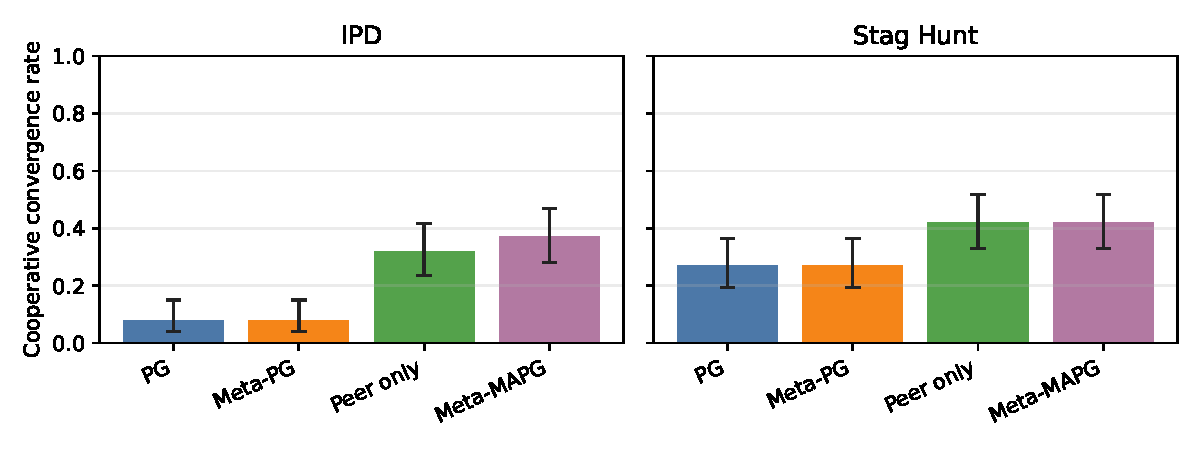
\includegraphics[width=\linewidth]{figures/ablation_success.pdf}
  \caption{Component ablation with Wilson $95\%$ confidence intervals over $100$ seeds. Peer-aware methods (peer-only, Meta-MAPG) separate from non-peer methods (PG, Meta-PG) in both games. Peer-only and full Meta-MAPG are not distinguishable within CIs; the claim is the peer-learning effect, not strict dominance of the full method.}
  \label{fig:ablation}
\end{figure}

\begin{figure}[t]
  \centering
  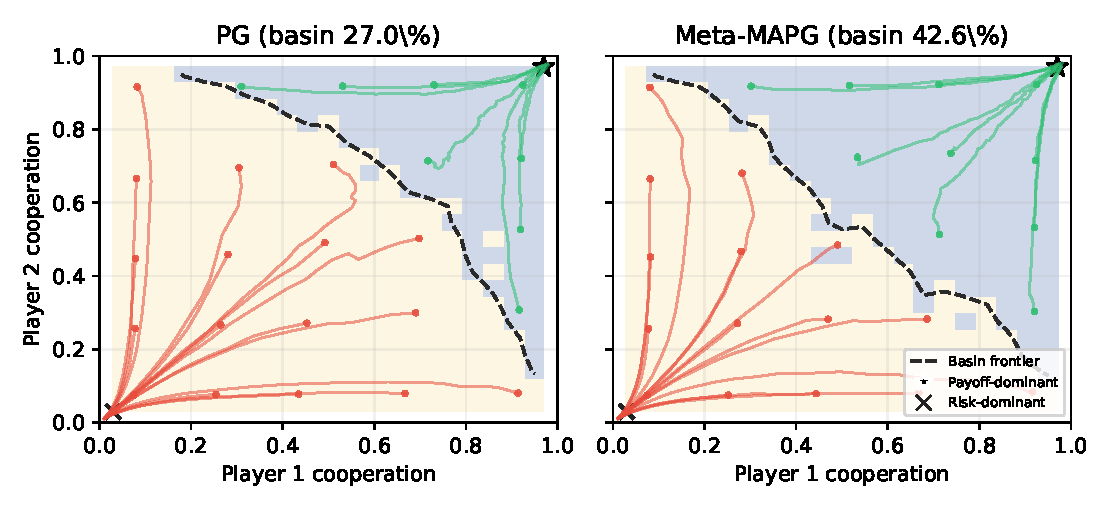
\includegraphics[width=\linewidth]{figures/basin_trajectories.pdf}
  \caption{Basin geometry and dynamics in Stag Hunt. Background shading is the empirical basin map on a $21\times21$ grid (lavender = payoff-dominant, cream = risk-dominant). The dashed contour is the empirical separatrix. Overlaid trajectories start from a $5\times5$ sub-grid; green curves succeed, red curves fail. Meta-MAPG pushes the frontier left and down: the cooperative basin grows from $27.0\%$ under PG to $42.6\%$, consistent with \cref{prop:basin}.}
  \label{fig:basin-traj}
\end{figure}

\begin{figure}[t]
  \centering
  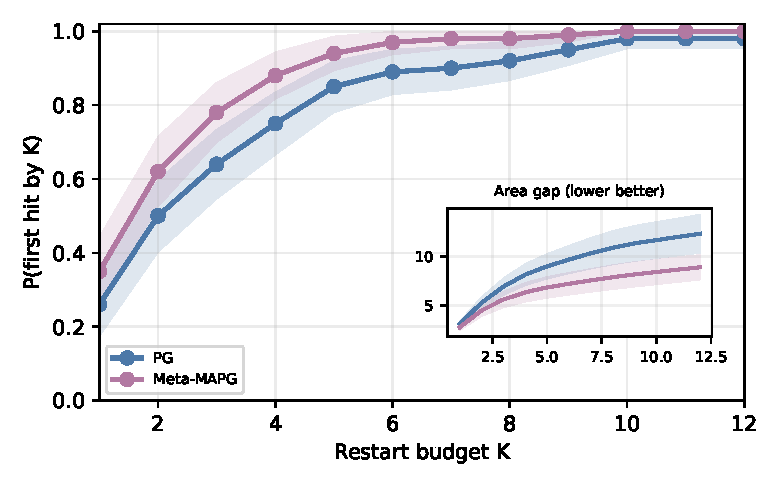
\includegraphics[width=\linewidth]{figures/restart_selection.pdf}
  \caption{Restart budget as equilibrium-selection budget in Stag Hunt. With paired restart initialisations, we plot the probability of discovering the payoff-dominant equilibrium by budget $K$; bands show 95\% confidence intervals. The inset shows $\sum_{k\le K}(8-W_k)$, the cumulative gap below best welfare (point estimates only, no CI band). Lower is better. Meta-MAPG reaches the good basin with fewer restarts.}
  \label{fig:restart}
\end{figure}

\begin{figure}[t]
  \centering
  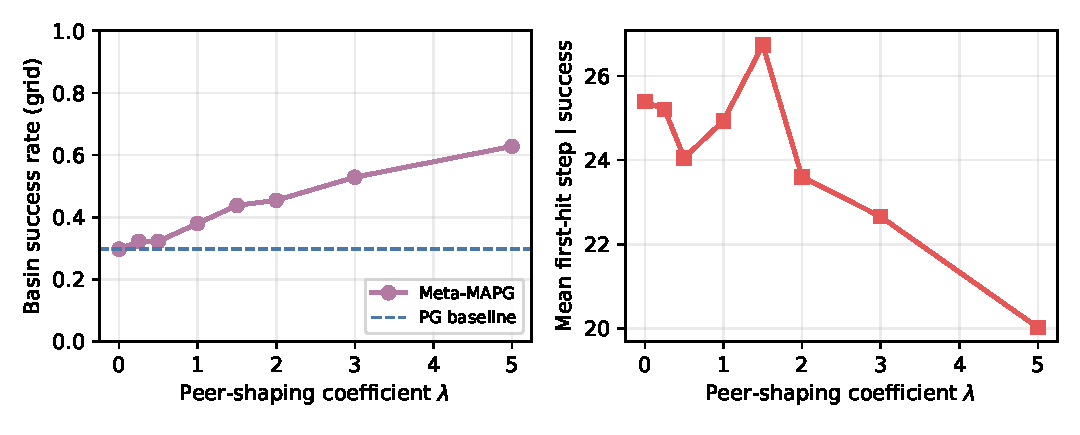
\includegraphics[width=\linewidth]{figures/peer_sweep.pdf}
  \caption{Peer-shaping sweep on Stag Hunt. Left: payoff-dominant basin fraction on an $11\times 11$ initial-policy grid as peer coefficient $\lambda$ varies. The rate grows from the PG baseline ($29.8\%$) to $62.8\%$ at $\lambda=5$, roughly linearly for small $\lambda$, as predicted by $\rho_\lambda\gtrsim\rho_0+\lambda\mu_M/(2L)$. Right: conditional mean first-hit step contracts from $\approx 25$ to $\approx 20$, matching \cref{cor:speedup}.}
  \label{fig:peer-sweep}
\end{figure}

\begin{figure}[t]
  \centering
  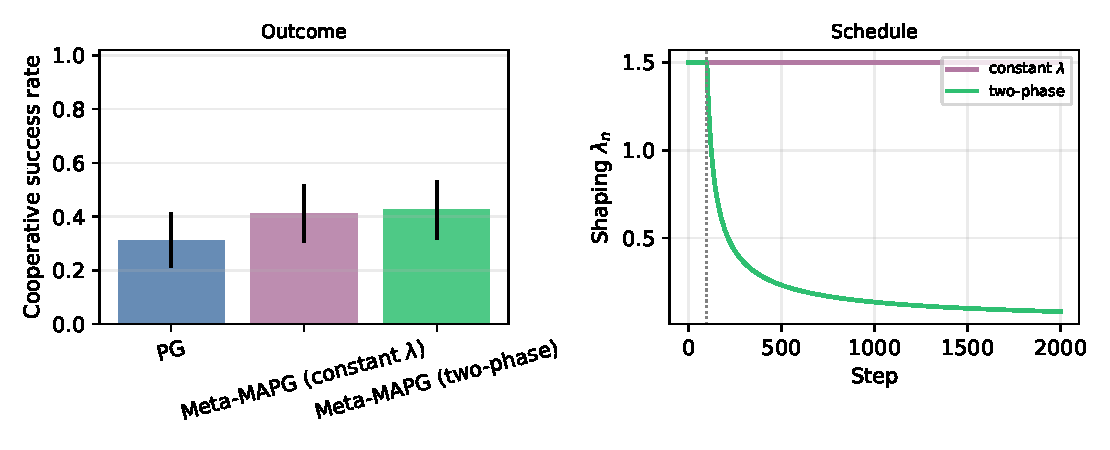
\includegraphics[width=\linewidth]{figures/annealing_ablation.pdf}
  \caption{Two-phase schedule vs constant shaping in tabular Stag Hunt ($80$ seeds, $2000$ steps, $\lambda_c=1.5$). PG reaches $31.25\%$, constant-shaping Meta-MAPG reaches $41.25\%$, and the two-phase schedule reaches $42.50\%$; second-half cooperation std is $\le 5\times10^{-4}$ in all three, so this tabular setting shows no measurable endpoint drift over the plotted horizon. The honest reading is therefore that the two-phase schedule is theoretical insurance for Nash consistency rather than an empirically separated effect in Stag Hunt. Appendix~\ref{app:mlp} reports the corresponding non-tabular MLP-IPD comparison. Right: $\lambda_n$ over time; the dotted line marks $N_0=100$.}
  \label{fig:annealing}
\end{figure}

\begin{table}[t]
  \centering
  \caption{Main 100-seed summary. Cooperative success uses a minimum initial-state cooperation threshold of $0.82$. Restart success and mean restarts are reported for all methods using paired restart initialisations.}
  \label{tab:results}
  \resizebox{\linewidth}{!}{\begin{tabular}{llccc}\toprule
Game & Method & Ablation success & Restart success & Restarts \\\midrule
stag hunt & PG & 27\% & 100\% & 1.71 \\
stag hunt & Meta-PG & 27\% & 100\% & 1.75 \\
stag hunt & Peer only & 42\% & 100\% & 1.24 \\
stag hunt & Meta-MAPG & 42\% & 100\% & 1.24 \\
ipd & PG & 8\% & 51\% & 8.68 \\
ipd & Meta-PG & 8\% & 57\% & 7.90 \\
ipd & Peer only & 32\% & 97\% & 2.91 \\
ipd & Meta-MAPG & 37\% & 100\% & 2.13 \\
\bottomrule
\end{tabular}
}
\end{table}

The ablation shows that peer-learning terms matter; it does not show that full Meta-MAPG dominates every LOLA-style variant. Peer-only and full Meta-MAPG are indistinguishable within CIs in both Stag Hunt ($42\%$ vs $42\%$, $1.24$ vs $1.24$ restarts) and IPD ($32\%$ vs $37\%$ within Wilson CI), so the empirical opponent-aware signal reduces to the peer term; disentangling the own-term likely requires longer unrolls (an $L\in\{1,3,5\}$ sweep in IPD is a natural follow-up). The trajectory figure shows the finite-time mechanism: opponent-aware shaping changes the local flow where the basin map changes. The restart-budget, basin, and peer-sweep experiments support \cref{thm:two-phase,thm:restart,prop:basin,cor:speedup}: restarts turn local convergence into equilibrium search, and shaping improves that search by increasing cooperative basin mass and first-passage probability. \Cref{fig:annealing} runs the two-phase schedule directly. It shows that annealing after $N_0$ steps preserves basin-entry performance while restoring the Nash target. The MLP-policy IPD check in \cref{app:mlp} is a transfer check, not a deep-MARL benchmark. The estimator sanity check in \cref{app:sanity} is not a proof of \cref{as:decomp}; it checks that the sample estimator moves in the predicted direction as batch size grows.

\section{Discussion}

The theorem is local first. Meta-MAPG inherits Giannou et al.'s stable-Nash theory only inside attracting neighbourhoods and only after the estimator has stochastic-approximation form. The two-phase theorem fixes the algorithmic role: constant shaping is for basin entry; annealing restores the original Nash target. Restarts search across basins. Selecting the best endpoint makes restart budget an equilibrium-selection resource. Its cost depends on basin probability $p_\rho$; shaping helps only when it increases that probability.

The assumptions are real. The estimator must have bounded conditional variance. Truncation must make unroll bias summable. Asymptotic shaping must be Nash-consistent. Constant shaping is useful for basin geometry, but a constant peer term can move fixed points in general-sum games. This is why the theorem separates annealed convergence from constant-shaping diagnostics.

The experiments are deliberately limited. Matrix and tabular games let us measure the theorem's objects: basins, restarts, drift, and estimator variance. Naive random restarts degrade with dimension: a radius-$\rho$ basin inside a radius-$R$ search region has worst-case mass $(\rho/R)^d$. Deep MARL needs stronger variance control, opponent models, differentiable longer unrolls, and structured restarts such as warm starts around high-welfare policies, possibly with DiCE-style estimators \citep{foerster2018dice}. The claim here is narrower: opponent-aware gradients can fit stochastic approximation, and basin-entry efficiency is the right global metric when convergence is local.

We do not claim unconditional convergence of arbitrary opponent-aware learning in deep MARL. We show that finite-unroll Meta-MAPG fits classical stochastic approximation under boundedness, smoothness, Nash-consistency, and summability assumptions. Independent restarts globalise the local result when local basin mass is positive. The MLP-policy check in \cref{app:mlp} only tests whether the peer-vs-nonpeer separation survives a modest neural parameterisation.

\appendix

\section{Proof of \texorpdfstring{\cref{lem:decomp}}{Lemma 4.1}}\label{app:decomp}

For a sampled trajectory $\tau$, write $S_i(\tau)=\nabla_{\phi_i}\log p_\phi(\tau)$, $H_i(\tau)=\nabla_{\phi_i}^2\log p_\phi(\tau)$, and let $R_i(\tau)$ be agent $i$'s discounted return.

\paragraph{Current term.}
The likelihood-ratio identity \citep{williams1992simple,sutton2018reinforcement} gives the single-sample estimator
$\widehat G_i^{\mathrm{cur}}(\tau):=R_i(\tau)S_i(\tau)$ with $\E[\widehat G_i^{\mathrm{cur}}\mid\F_n]=\nabla_{\phi_i}J_i(\phi_n)$.

\paragraph{Own-learning term.}
Differentiating $J_i(\phi_i+\eta\nabla_{\phi_i}J_i,\phi_{-i})$ in $\phi_i$ yields
$\nabla_{\phi_i}J_i+\eta[\nabla_{\phi_i}^2J_i]^\top\nabla_{\phi_i}J_i$, and the Hessian identity
\[
\nabla_{\phi_i}^2J_i
=\E\!\left[R_i(\tau)\!\left(S_i(\tau)S_i(\tau)^\top+H_i(\tau)\right)\right]
\]
gives the single-sample estimator
$\widehat G_i^{\mathrm{own}}(\tau):=\eta\,\widehat H_{ii}(\tau)^\top\widehat G_i^{\mathrm{cur}}(\tau)$.

\paragraph{Peer-learning term.}
For $\phi_j'=\phi_j+\eta\nabla_{\phi_j}J_j$, differentiating $J_i(\phi_i,\phi_j')$ in $\phi_i$ contributes
\[
\eta\bigl[\nabla_{\phi_i}\nabla_{\phi_j}J_j\bigr]^\top\nabla_{\phi_j}J_i.
\]
Under per-agent parameterisation $S_j$ has no $\phi_i$-dependence, so the mixed likelihood-ratio identity collapses to
\[
\nabla_{\phi_i}\nabla_{\phi_j}J_j
=\E\!\left[R_j(\tau)S_j(\tau)S_i(\tau)^\top\right],
\]
yielding $\widehat G_i^{\mathrm{peer}}(\tau):=\eta\,\widehat C_{ji}(\tau)^\top\widehat G_j^{\mathrm{cur}}(\tau)$.

\paragraph{Martingale noise and truncation bias.}
Each of $\widehat G_i^{\mathrm{cur}},\widehat G_i^{\mathrm{own}},\widehat G_i^{\mathrm{peer}}$ is a polynomial in the bounded-second-moment quantities $R_i,R_j,S_i,S_j,H_i$, hence has finite conditional second moment on $\K$. Setting
\[
\xi_{n+1}^{\bullet}:=\widehat G_i^{\bullet}-\E[\widehat G_i^{\bullet}\mid\F_n],\quad \bullet\in\{\mathrm{cur},\mathrm{own},\mathrm{peer}\},
\]
each is a martingale difference with bounded conditional variance; so is their sum $\xi_{n+1}$. Longer unrolls repeat this chain-rule structure across $L_n$ inner updates, and the truncated-tail plus approximate-opponent modelling residual is deterministic given $\F_n$. Collecting it into $b_n:=\E[g_n\mid\F_n]-F(\phi_n)$, the bounded-derivative hypotheses on $\K$ and \cref{as:trunc} give $\|b_n\|\le C\beta_n$ with $\beta_n\to0$. Assembling the three components produces
\[
g_n=F(\phi_n)+b_n+\xi_{n+1},
\]
which is exactly \cref{as:decomp}. $\square$

\section{Local Lyapunov Drift}\label{app:lyapunov}

We spell out the stochastic-approximation step behind \cref{lem:local}. The goal is not to reprove \citet{giannou2022convergence}; it is to show that Meta-MAPG has the same Lyapunov form after decomposition.

\begin{lemma}[One-step local Lyapunov drift]\label{lem:app-lyapunov}
Fix an SOS Nash equilibrium $\phi^\ast$ and a ball $\B_\rho=\{\phi:\|\phi-\phi^\ast\|\le\rho\}$ on which the effective field $F$ satisfies
\[
\langle F(\phi),\phi-\phi^\ast\rangle\le -\mu\|\phi-\phi^\ast\|^2 .
\]
Suppose the stopped iterates remain in $\B_\rho$ and the Meta-MAPG update admits
\[
\begin{gathered}
g_n=F(\phi_n)+\xi_{n+1}+b_n,\\
\E[\xi_{n+1}\mid\F_n]=0,\qquad
\E[\|\xi_{n+1}\|^2\mid\F_n]\le\sigma^2,
\end{gathered}
\]
with $\|b_n\|\le\beta_n$. If $V_n=\|\phi_n-\phi^\ast\|^2$ and $\|F(\phi)\|\le C_F$ on $\B_\rho$, then
\begin{equation}\label{eq:local-lyap}
\begin{aligned}
\E[V_{n+1}\mid\F_n]
&\le (1-2\mu\alpha_n)V_n
   +2\alpha_n\beta_n\sqrt{V_n}\\
&\quad+3\alpha_n^2(C_F^2+\beta_n^2+\sigma^2).
\end{aligned}
\end{equation}
\end{lemma}

\begin{proof}
Projection onto the convex compact set $\K$ is non-expansive, so it is enough to bound the unprojected step. Expanding the square gives
\[
\begin{aligned}
V_{n+1}
&\le \|\phi_n-\phi^\ast+\alpha_n g_n\|^2\\
&=V_n+2\alpha_n\langle g_n,\phi_n-\phi^\ast\rangle
  +\alpha_n^2\|g_n\|^2 .
\end{aligned}
\]
Taking conditional expectation and using $\E[\xi_{n+1}\mid\F_n]=0$,
\[
\begin{aligned}
\E[\langle g_n,\phi_n-\phi^\ast\rangle\mid\F_n]
&=\langle F(\phi_n),\phi_n-\phi^\ast\rangle\\
&\quad+\langle b_n,\phi_n-\phi^\ast\rangle\\
&\le -\mu V_n+\beta_n\sqrt{V_n}.
\end{aligned}
\]
For the quadratic term, $(a+b+c)^2\le 3(a^2+b^2+c^2)$ gives
\[
\begin{aligned}
\E[\|g_n\|^2\mid\F_n]
&\le 3\bigl(\|F(\phi_n)\|^2+\|b_n\|^2\\
&\quad+\E[\|\xi_{n+1}\|^2\mid\F_n]\bigr)\\
&\le 3(C_F^2+\beta_n^2+\sigma^2).
\end{aligned}
\]
Substituting the last two displays into the square expansion proves \eqref{eq:local-lyap}.
\end{proof}

If $\sum_n\alpha_n\beta_n<\infty$ and $\sum_n\alpha_n^2<\infty$, then \eqref{eq:local-lyap} is in Robbins--Siegmund form. Indeed,
\[
2\alpha_n\beta_n\sqrt{V_n}\le \alpha_n\beta_n(1+V_n),
\]
so for all large $n$,
\[
\E[V_{n+1}\mid\F_n]\le (1-a_n)V_n+\eta_n
\]
with $\sum_n a_n=\infty$ and $\sum_n\eta_n<\infty$. Robbins--Siegmund yields $V_n\to V_\infty$ almost surely and $\sum_n a_nV_n<\infty$; since $\sum_n a_n=\infty$, $V_\infty=0$. Thus $\phi_n\to\phi^\ast$ almost surely on the local event.

\section{Proof of Proposition~\ref{prop:basin}}\label{app:prop-basin}

We prove the three parts separately.

\paragraph{Fixed-point shift.}
$F_\lambda(\phi^\ast)=\lambda M(\phi^\ast)$, where $M(\phi^\ast)=M^{\mathrm{peer}}(\phi^\ast)\ne0$ in general (own-learning vanishes because $\nabla_{\phi_i}J_i(\phi^\ast)=0$). Since $J_v=Dv(\phi^\ast)$ is non-singular under SOS, the implicit function theorem applied to $\Phi(\lambda,\phi):=F_\lambda(\phi)$ at $(0,\phi^\ast)$ gives a $C^1$ branch $\phi^\ast_\lambda$ with $F_\lambda(\phi^\ast_\lambda)=0$ and
\[
\phi^\ast_\lambda=\phi^\ast-\lambda J_v^{-1}M(\phi^\ast)+O(\lambda^2),
\]
so $\|\phi^\ast_\lambda-\phi^\ast\|=O(\lambda)$ for small $\lambda$.

\paragraph{Linearised drift bound.}
Both $J_v$ and $J_M$ are real matrices; their symmetric parts $\operatorname{sym}(A):=(A+A^\top)/2$ are Hermitian. By definition $-\lambda_{\max}(\operatorname{sym}(J_v))=\mu$ and $-\lambda_{\max}(\operatorname{sym}(J_M))=\mu_M$. Because $DM(\phi^\ast_\lambda)=DM(\phi^\ast)+O(\|\phi^\ast_\lambda-\phi^\ast\|)=J_M+O(\lambda)$, the shaping Jacobian evaluated at the shifted fixed point differs from $J_M$ by $O(\lambda)$, which becomes an $O(\lambda^2)$ contribution after multiplying by $\lambda$. Thus $DF_\lambda(\phi^\ast_\lambda)=J_v+\lambda J_M+O(\lambda^2)$. Weyl's inequality gives
\[
\lambda_{\max}\!\bigl(\operatorname{sym}(J_v+\lambda J_M)\bigr)\le \lambda_{\max}\!\bigl(\operatorname{sym}(J_v)\bigr)+\lambda\,\lambda_{\max}\!\bigl(\operatorname{sym}(J_M)\bigr),
\]
and negating, together with the $O(\lambda^2)$ evaluation shift, yields \eqref{eq:weyl}.

\paragraph{Certified radius.}
Let $\mu_\lambda:=\mu+\lambda\mu_M$. Fix $\phi\in\B_{\rho_\lambda}(\phi^\ast_\lambda)$ and write $x:=\phi-\phi^\ast_\lambda$. Since $F_\lambda(\phi^\ast_\lambda)=0$, Taylor's theorem with integral remainder gives
\[
F_\lambda(\phi)=J_\lambda x+R_\lambda(x),\qquad \|R_\lambda(x)\|\le\tfrac{1}{2}L_\lambda\|x\|^2,
\]
with $J_\lambda=DF_\lambda(\phi^\ast_\lambda)$ and $L_\lambda$ the Lipschitz constant of $DF_\lambda$ on $\B_{\rho_\lambda}(\phi^\ast_\lambda)$. Taking inner products,
\[
\langle J_\lambda x,x\rangle=x^\top\operatorname{sym}(J_\lambda)x\le -\mu_\lambda\|x\|^2
\]
by Rayleigh and \eqref{eq:weyl} (absorbing the $O(\lambda^2)$ term into $\mu_\lambda$ for small $\lambda$), and $|\langle R_\lambda(x),x\rangle|\le\tfrac{1}{2}L_\lambda\|x\|^3$. Hence
\[
\langle F_\lambda(\phi),\phi-\phi^\ast_\lambda\rangle\le-\mu_\lambda\|x\|^2+\tfrac{1}{2}L_\lambda\|x\|^3.
\]
For $\|x\|\le\rho_\lambda:=\mu_\lambda/(2L_\lambda)$, the cubic term is at most $(\mu_\lambda/4)\|x\|^2$, so
\[
\langle F_\lambda(\phi),\phi-\phi^\ast_\lambda\rangle\le-\tfrac{1}{2}\mu_\lambda\|x\|^2,
\]
the stated SOS drift on $\B_{\rho_\lambda}(\phi^\ast_\lambda)$. $\square$

\section{Proof of Theorem~\ref{thm:two-phase}}\label{app:thm-twophase}

Write $V_n=\|\phi_n-\phi^\ast_{\lambda_c}\|^2$ (phase-1 Lyapunov, centred at the shifted fixed point of \cref{prop:basin}) and let $\tau:=\inf\{n\le N_0:\phi_n\notin\B_\rho\}$ with $\tau=N_0+1$ if the iterates never leave. On the event $\{n<\tau\}$ the phase-1 drift of \cref{prop:basin} applies with constant $\mu_{\lambda_c}$.

\paragraph{Step 1: one-step drift.}
On $\{n<\tau\}$, by \cref{as:decomp} and the phase-1 drift bound around $\phi^\ast_{\lambda_c}$,
\[
\begin{aligned}
\E[V_{n+1}\mid\F_n]
&=\E\!\left[\|\phi_n-\phi^\ast_{\lambda_c}+\alpha_0 g_n\|^2\mid\F_n\right]\\
&=V_n+2\alpha_0\langle F_{\lambda_c}(\phi_n),\phi_n-\phi^\ast_{\lambda_c}\rangle\\
&\quad+2\alpha_0\langle b_n,\phi_n-\phi^\ast_{\lambda_c}\rangle+\alpha_0^2\E[\|g_n\|^2\mid\F_n]\\
&\le V_n-2\alpha_0\mu_{\lambda_c}V_n
+2\alpha_0\beta_0\sqrt{V_n}+\alpha_0^2 G^2,
\end{aligned}
\]
where $G^2:=3(C_{F_{\lambda_c}}^2+\beta_0^2+\sigma^2)$ is a uniform bound on the conditional second moment of $g_n$ (with $C_{F_{\lambda_c}}$ the sup-norm of $F_{\lambda_c}$ on $\B_\rho$). Applying $2a b\le \eta a^2+\eta^{-1}b^2$ with $a=\sqrt{V_n}$, $b=\beta_0$, and $\eta=\mu_{\lambda_c}$,
\[
\E[V_{n+1}\mid\F_n]\le (1-\mu_{\lambda_c}\alpha_0)V_n
+\frac{\alpha_0\beta_0^2}{\mu_{\lambda_c}}+\alpha_0^2 G^2.
\]

\paragraph{Step 2: unconditional recursion on the stopped process.}
Define the stopped sequence $\tilde V_n:=V_{n\wedge\tau}$. The drift bound and the fact that $\tilde V_{n+1}=\tilde V_n$ on $\{n\ge\tau\}$ give
\[
\begin{aligned}
\E[\tilde V_{n+1}]
&\le (1-\mu_{\lambda_c}\alpha_0)\E[\tilde V_n]+c_1,\\
c_1&:=\frac{\alpha_0\beta_0^2}{\mu_{\lambda_c}}+\alpha_0^2G^2.
\end{aligned}
\]
Iterating,
\[
\E[\tilde V_{N_0}]\le (1-\mu_{\lambda_c}\alpha_0)^{N_0}V_0+\frac{c_1}{\mu_{\lambda_c}\alpha_0}.
\]
Using $(1-x)^k\le e^{-xk}$ for $x\in[0,1]$,
\[
\E[\tilde V_{N_0}]\le V_0\,e^{-\mu_{\lambda_c}\alpha_0 N_0}+\frac{\beta_0^2}{\mu_{\lambda_c}^2}+\frac{\alpha_0 G^2}{\mu_{\lambda_c}}.
\]

\paragraph{Step 3: Markov's inequality.}
If $\phi_{N_0}\notin\B_{\rho/2}$ and $\tau>N_0$, then $V_{N_0}\ge(\rho/2)^2$. If instead $\tau\le N_0$, then by definition of $\tau$ we have $\phi_\tau\notin\B_\rho$, so $V_\tau>\rho^2\ge(\rho/2)^2$, and the stopped process freezes at $\tilde V_{N_0}=V_\tau$. Hence in both cases $\tilde V_{N_0}\ge(\rho/2)^2$. Therefore
\[
\begin{aligned}
&\Pr(\phi_{N_0}\notin\B_{\rho/2}\mid \phi_0\in\B_\rho)\\
&\quad\le \Pr(\tilde V_{N_0}\ge (\rho/2)^2)
\le \frac{4\E[\tilde V_{N_0}]}{\rho^2}.
\end{aligned}
\]
Combining with Step 2,
\[
\begin{aligned}
&\Pr(\phi_{N_0}\notin\B_{\rho/2}\mid\phi_0\in\B_\rho)\\
&\quad\le \frac{4}{\rho^2}\!\left(
V_0 e^{-\mu_{\lambda_c}\alpha_0 N_0}
+C\alpha_0(\beta_0^2+\alpha_0\sigma^2)\right),
\end{aligned}
\]
for a constant $C$ depending on $\mu_{\lambda_c}$, $C_{F_{\lambda_c}}$.

\paragraph{Step 4: choice of $N_0$.}
Given a target $\delta\in(0,1)$, set
\[
N_0=\left\lceil\frac{1}{\mu_{\lambda_c}\alpha_0}\log\!\frac{8V_0}{\delta\rho^2}\right\rceil,
\qquad \alpha_0\le \frac{\delta\rho^2}{8C(\beta_0^2+\sigma^2)}.
\]
Each summand in Step 3 is then at most $\delta/2$, so the total failure probability is at most $\delta$.

\paragraph{Step 5: phase 2.}
Conditional on $\phi_{N_0}\in\B_{\rho/2}$, the subsequent recursion uses $\alpha_n=\alpha_0 n^{-p}$ and $\lambda_n=\lambda_c n^{-q}$ with $1/2<p\le 1$ and $q>1-p$, so $\sum_n\alpha_n=\infty$, $\sum_n\alpha_n^2<\infty$, and $\sum_n\alpha_n\lambda_n<\infty$ by direct integral comparison. By the triangle inequality and the explicit shift bound in \cref{thm:two-phase},
\[
\|\phi_{N_0}-\phi^\ast\|
\le
\|\phi_{N_0}-\phi^\ast_{\lambda_c}\|+\|\phi^\ast_{\lambda_c}-\phi^\ast\|
\le
\frac{\rho}{2}+c_{\mathrm{shift}}\lambda_c
\le
\frac{3\rho}{4}
<r_{\mathrm{att}}.
\]
Hence the phase-2 iterate starts inside the attracting radius of \cref{lem:local}. The annealed fixed-point branch satisfies $\phi^\ast_{\lambda_n}\to\phi^\ast$ by \cref{prop:basin}; together with \cref{as:trunc,as:decomp,as:stable}, this places the recursion inside the hypotheses of \cref{lem:local} on the event $\{\phi_{N_0}\in\B_{\rho/2}\}$. Conditional on this event, $\phi_n\to\phi^\ast$ almost surely. The total probability that the two-phase procedure converges in a single epoch is therefore at least $(1-\delta)\cdot 1=1-\delta$. $\square$

\section{Proof of Theorem~\ref{thm:restart}}\label{app:thm-restart}

Let $\F_k^{\mathrm{epoch}}$ denote the $\sigma$-algebra generated by epochs $1,\ldots,k-1$ (outcomes only; restart draws are independent by assumption). Let $A_k$ be the event that epoch $k$ starts in $\B_\rho$ and that the two-phase procedure of \cref{thm:two-phase} reaches phase 2 and converges within that epoch.

\paragraph{Step 1: per-epoch lower bound.}
Restart $k$ samples $\phi_0^{(k)}\sim\nu$ independently of $\F_k^{\mathrm{epoch}}$, so
\[
\Pr(\phi_0^{(k)}\in\B_\rho\mid\F_k^{\mathrm{epoch}})=\nu(\B_\rho)=p_\rho.
\]
Conditional on $\phi_0^{(k)}\in\B_\rho$, \cref{thm:two-phase} gives $\Pr(\text{epoch succeeds})\ge 1-\delta$. Therefore
\[
\Pr(A_k\mid\F_k^{\mathrm{epoch}})\ge p_\rho(1-\delta)=:p_\star>0.
\]

\paragraph{Step 2: geometric tail.}
Let $T:=\inf\{k\ge 1:A_k\text{ occurs}\}$. Then
\[
\begin{aligned}
\Pr(T>k)
&=\E\!\left[\prod_{j=1}^k\mathbf{1}_{A_j^c}\right]\\
&=\E\!\left[
\E[\mathbf{1}_{A_k^c}\mid\F_k^{\mathrm{epoch}}]
\prod_{j=1}^{k-1}\mathbf{1}_{A_j^c}\right].
\end{aligned}
\]
By Step 1, $\E[\mathbf{1}_{A_k^c}\mid\F_k^{\mathrm{epoch}}]\le 1-p_\star$ almost surely, so iterating,
\[
\Pr(T>k)\le (1-p_\star)^k.
\]
Hence $\Pr(T<\infty)=1$ and
\[
\E[T]=\sum_{k\ge 0}\Pr(T>k)\le \sum_{k\ge 0}(1-p_\star)^k=\frac{1}{p_\star}.
\]

\paragraph{Step 3: dimensional dependence.}
If $\nu$ is lower-bounded by density $m>0$ on a neighbourhood $U_{\lambda_c}$ containing $\B_\rho(\phi^\ast_{\lambda_c})$ in $\R^d$, then $p_\rho\ge m\,c_d\rho^d$ where $c_d=\pi^{d/2}/\Gamma(d/2+1)$ is the volume of the unit $d$-ball. Because $\|\phi^\ast_{\lambda_c}-\phi^\ast\|=O(\lambda_c)$, for sufficiently small $\lambda_c$ this is the same local region as a neighbourhood of $\phi^\ast$ up to shrinking $U_{\lambda_c}$ by an $O(\lambda_c)$ margin. Combined with the certified radius $\rho_\lambda\ge (\mu+\lambda\mu_M)/(2L_\lambda)$ from \cref{prop:basin}, the expected number of epochs obeys
\[
\E[T]\le \frac{1}{(1-\delta)m c_d}\!\left(\frac{2L_\lambda}{\mu+\lambda\mu_M}\right)^{\!d}.
\]
Shaping reduces the base of this dimensional factor whenever $\mu_M>0$; the overall worst-case dependence is still exponential in $d$, as discussed in \cref{sec:main}. $\square$

\section{Experiment Reproducibility}\label{app:repro}

The experiment scripts, figures, CSVs, and run configurations are included. The tabular script saves its command-line configuration and outputs under \texttt{artifacts/main}. These files cover the ablation, restart, trajectory, basin, peer-sweep, annealing, and estimator-sanity figures. Updates use no exact gradients; expected returns are computed only for logging and evaluation.

The optional MLP-policy IPD check in \cref{app:mlp} requires PyTorch and uses DiCE-style surrogate losses for the higher-order terms. Its aggregate ablation and annealing outputs are stored under \texttt{artifacts/mlp}, including \texttt{mlp\_ipd.pdf}, \texttt{mlp\_annealing.pdf}, and their per-seed summary CSVs. The repository README contains the full commands for regenerating both sets of experiments.

\section{Non-Tabular IPD Check}\label{app:mlp}

To check that the ablation is not purely tabular, we repeat IPD with a two-layer MLP policy for each agent: a 5-dimensional one-hot previous-action input, two tanh hidden layers of width 16, and one Bernoulli cooperation logit. This scales the policy from 5 tabular logits to about 385 parameters per agent. We keep the tabular budget, batch size, seed schedule, peer coefficient, and own coefficient. Higher-order terms use PyTorch autograd with DiCE-style surrogate losses \citep{foerster2018dice}.

\begin{figure}[h]
  \centering
  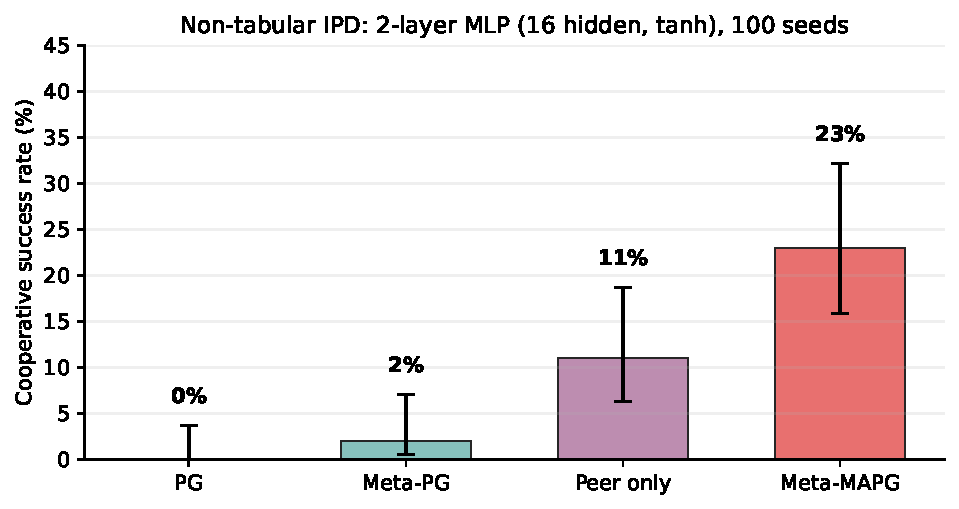
\includegraphics[width=0.82\linewidth]{figures/mlp_ipd.pdf}
  \caption{Non-tabular IPD check with MLP policies. Cooperative success rate over 100 seeds with Wilson 95\% confidence intervals. Peer-aware methods remain above non-peer methods under the same coefficients as the tabular experiments: PG reaches $0\%$, Meta-PG $2\%$, peer-only $11\%$, and Meta-MAPG $23\%$. This is a transfer check, not a deep-MARL benchmark.}
  \label{fig:mlp-ipd}
\end{figure}

We also mirror the annealing comparison in the same MLP IPD setting. The point is not to claim a large non-tabular gain from the schedule; it is to check that the two-phase construction does not collapse once the policy is no longer tabular.

\begin{figure}[h]
  \centering
  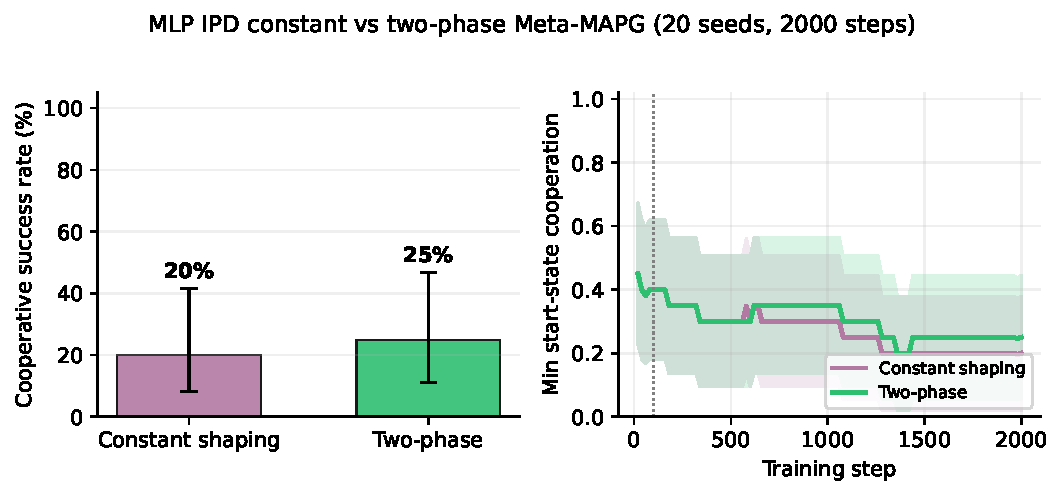
\includegraphics[width=0.98\linewidth]{figures/mlp_annealing.pdf}
  \caption{Constant shaping vs two-phase Meta-MAPG in MLP IPD ($20$ seeds, $2000$ steps, $N_0=100$). Left: cooperative success rate with Wilson $95\%$ confidence intervals. Constant shaping reaches $20\%$ and two-phase reaches $25\%$, so the separation is small but directionally aligned with the tabular story. Right: mean minimum start-state cooperation over training, with the dotted line marking the end of phase~1. The non-tabular comparison therefore supports the narrower claim needed by \cref{thm:two-phase}: annealing does not materially harm basin-entry performance, even when the policy class is an MLP.}
  \label{fig:mlp-annealing}
\end{figure}

\section{Estimator Sanity Check}\label{app:sanity}

\begin{figure}[h]
  \centering
  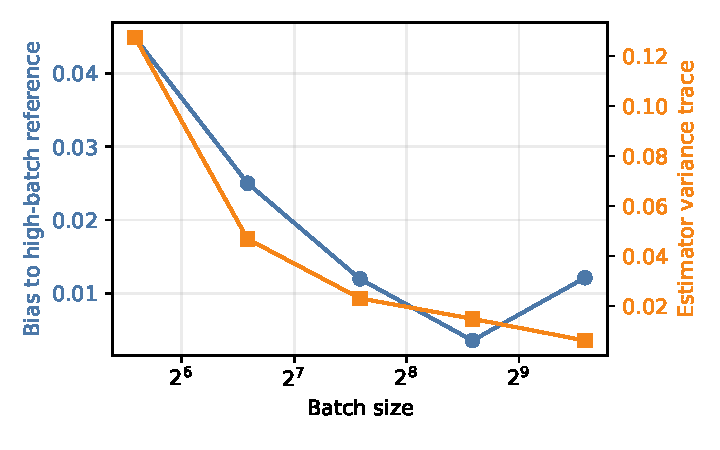
\includegraphics[width=0.78\linewidth]{figures/estimator_sanity.pdf}
  \caption{Estimator sanity check. At a fixed Stag Hunt parameter, the variance trace of the Meta-MAPG estimator decreases from $0.1272$ at batch size $48$ to $0.0062$ at batch size $768$. Bias is measured relative to a high-batch reference estimator, not an exact analytic gradient.}
  \label{fig:sanity}
\end{figure}

\bibliography{references}

\end{document}
